\section{Порядок выполнения лабораторной работы \No1}
\refstepcounter{chapter}
\addcontentsline{toc}{chapter}{Приложение А Порядок выполнения лабораторной работы \No1}
\begin{enumerate}
\item Выбрать вариант задания в приложении \ref{Lab1Var} в соответствии с номером в журнале. 
\item Создать в папке с номером группы на рабочем столе папку \verb#Lab1# для файлов проекта.
\item Скопировать в созданную папку \verb#Lab1#, папку CMSIS из папки \verb#Лабораторные работы по микроконтроллерам/Materials# на рабочем столе.
\item Добавить в созданную папку с проектом папку \verb#STM32L1xx_StdPeriph_Driver# из папки \verb#Лабораторные работы по микроконтроллерам/Materials#.
\item Добавить в созданную папку с проектом файл \verb\stm32l1xx_conf.h\ из папки \verb#Лабораторные работы по микроконтроллерам/Materials#, добавить его в проект.
\item Добавьте в файлы \verb\stm32l1xx_gpio.c\, \verb\stm32l1xx_rcc.c\ строку:
\begin{verbatim}
#include <stm32l1xx_conf.h>
\end{verbatim}
\item Создать и настроить проект в среде разработки IAR. В качестве имени проекта указать \textit{lab1}, все файлы настроек проекта сохранить в папке \verb#Lab1#.
\item Добавить в проект IAR файлы \verb\stm32l1xx_gpio.c\, \verb\stm32l1xx_gpio.h\, \verb\stm32l1xx_rcc.c\, \verb\stm32l1xx_rcc.h\.
\item Построить блок-схему алгоритма главной программы.
\item Написать программу для микроконтроллера на языке Си.
\item Подключить отладочную плату STM32L - Discovery к компьютеру.
\item Загрузить программу в микроконтроллер и произвести ее отладку.
\item Отчет.
\end{enumerate}



\section{Пример выполнения лабораторной работы \No1}
Разработать программу для микроконтроллера в среде IAR и построить блок схему алгоритма главной программы. Работа светодиодов LD3 (Green) и LD4 (Blue) задается временными диаграммами. Последовательность, приведенная на временной диаграмме, должна повторяться бесконечно.
\begin{figure}[H]
\begin{center}
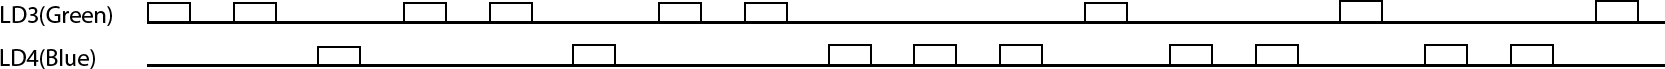
\includegraphics[scale=0.3]{Image/77.jpg} 
\end{center}
\caption{Временная диаграмма}
\end{figure}

\begin{figure}[H]
\begin{center}
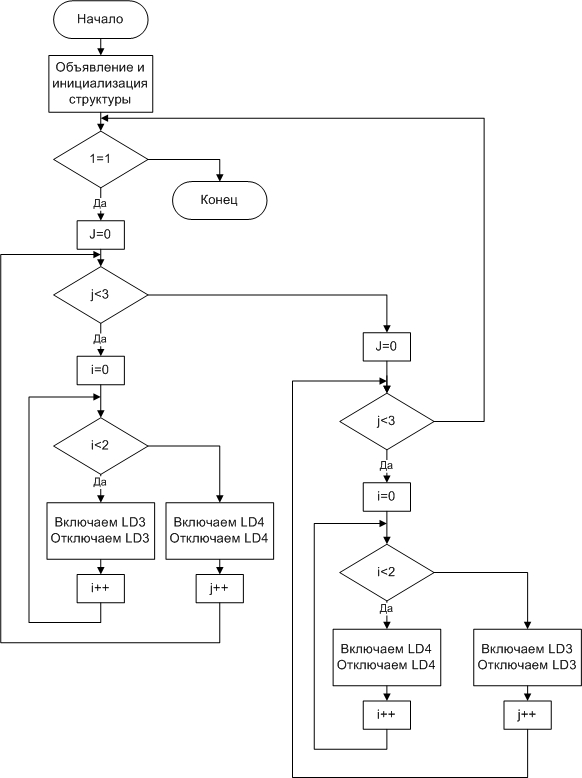
\includegraphics[scale=0.6]{Image/78.jpg} 
\end{center}
\caption{Схема алгоритма главной программы}
\end{figure}

\section{Пример главной программы для микроконтроллера}
\begin{verbatim}
#include <stm32l1xx.h>
#include <stm32l1xx_conf.h>
#include <stm32l1xx_gpio.h>
#include <stm32l1xx_rcc.h> 
void delay(int B); /*Прототип функции delay()*/
void led3(void);   /*Прототип функции led3()*/
void led4(void);   /*Прототип функции led4()*/

int main(void)
{
/*Объявление переменных типа uint32_t*/   
uint32_t i,j; 

/*Объявление структуры GPIO_InitStructure*/ 
GPIO_InitTypeDef GPIO_InitStructure; 
/*Включение тактирования*/
RCC_AHBPeriphClockCmd(RCC_AHBPeriph_GPIOB, ENABLE);   
GPIO_InitStructure.GPIO_Pin = GPIO_Pin_7 | GPIO_Pin_6 ;
GPIO_InitStructure.GPIO_Mode = GPIO_Mode_OUT;
GPIO_InitStructure.GPIO_Speed = GPIO_Speed_10MHz;
GPIO_InitStructure.GPIO_OType = GPIO_OType_PP;
/*Инициализация структуры*/        
GPIO_Init(GPIOB, &GPIO_InitStructure);  
  while (1)
  {
    j=0;
      while (j<3)
      {
        for (i=0;i<2;i++)
        led3();
        led4();
        j++;       
      }
    j=0;
      while (j<3)
     {
        for (i=0;i<2;i++)
        led4();
        led3();
        j++;       
      }         
  }
}
void delay(int B) /*Определение функции delay()*/
{
  int i;  
  for (i=0;i<=B;i++)
  ;
}
void led3(void)   /*Определение функции led3()*/
{
  GPIO_SetBits(GPIOB, GPIO_Pin_7);
  delay(100000);
  GPIO_ResetBits(GPIOB, GPIO_Pin_7);
  delay(100000);
}
void led4(void)   /*Определение функции led4()*/
{
  GPIO_SetBits(GPIOB, GPIO_Pin_6);
  delay(100000);
  GPIO_ResetBits(GPIOB, GPIO_Pin_6);
  delay(100000);
}
\end{verbatim}

\section{Варианты заданий к лабораторной работе \No1}
\label{Lab1Var}
\begin{figure}[H]
\begin{center}
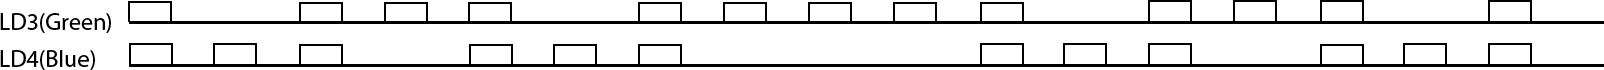
\includegraphics[scale=0.3]{Image/79.jpg} 
\end{center}
\caption{Вариант \No1}
\end{figure}
\begin{figure}[H]
\begin{center}
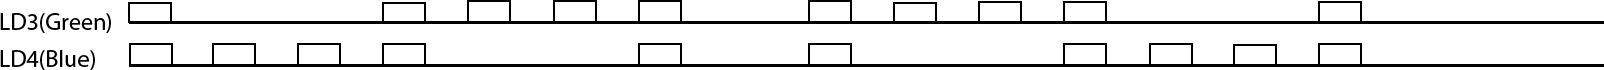
\includegraphics[scale=0.3]{Image/80.jpg} 
\end{center}
\caption{Вариант \No2}
\end{figure}
\begin{figure}[H]
\begin{center}
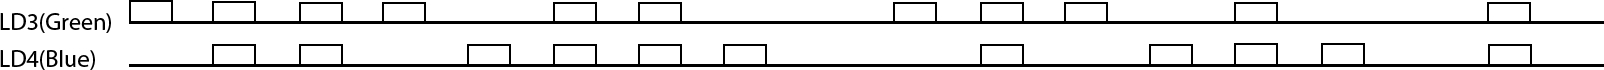
\includegraphics[scale=0.3]{Image/81.jpg} 
\end{center}
\caption{Вариант \No3}
\end{figure}
\begin{figure}[H]
\begin{center}
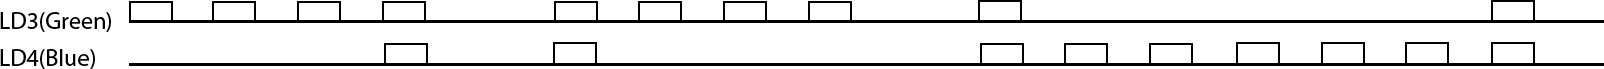
\includegraphics[scale=0.3]{Image/82.jpg} 
\end{center}
\caption{Вариант \No4}
\end{figure}
\begin{figure}[H]
\begin{center}
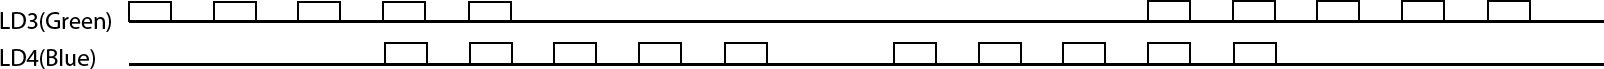
\includegraphics[scale=0.3]{Image/83.jpg} 
\end{center}
\caption{Вариант \No5}
\end{figure}
\begin{figure}[H]
\begin{center}
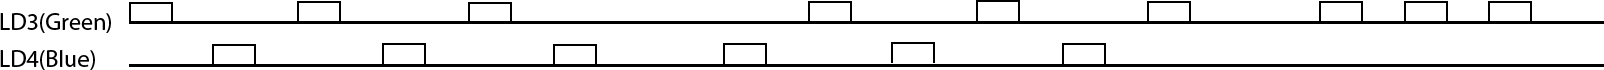
\includegraphics[scale=0.3]{Image/84.jpg} 
\end{center}
\caption{Вариант \No6}
\end{figure}
\begin{figure}[H]
\begin{center}
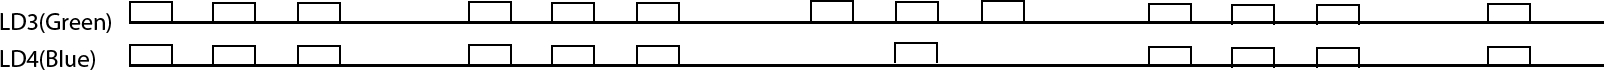
\includegraphics[scale=0.3]{Image/85.jpg} 
\end{center}
\caption{Вариант \No7}
\end{figure}
\begin{figure}[H]
\begin{center}
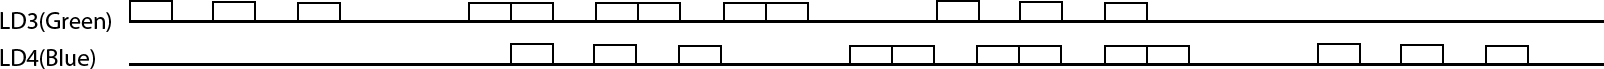
\includegraphics[scale=0.3]{Image/86.jpg} 
\end{center}
\caption{Вариант \No8}
\end{figure}
\begin{figure}[H]
\begin{center}
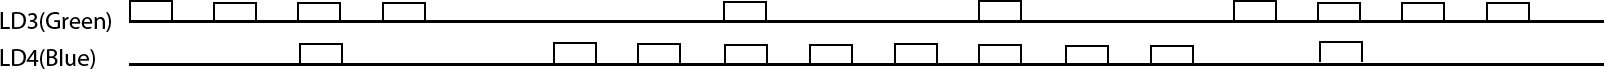
\includegraphics[scale=0.3]{Image/87.jpg} 
\end{center}
\caption{Вариант \No9}
\end{figure}